\section{Introduction}
The motivation for creating a package for the modelling of smooth transition
ARMA models was the observation that many phenomena appear to go
through different states which may be explained by some underlying and
observable factors.\footnote{As opposed to unobservable factors which leads to
a different class of models, such as the Markov switching models.}
In financial markets, under different states of the business cycle, financial
instruments have been observed to exhibit different characteristics with
recessions (or the lead up to such) usually marked by increased volatility and lower 
or negative mean. Being able to model the evolution of the process driving such 
changes and hence the switch from one state to another must surely make for a 
better understanding of the underlying dynamics and perhaps lead to a better
forecast model.

The precursor to smooth transition models appears to have been
\cite{Carmichael1928} who used the arctangent transformation to capture the
change in trends of a number of common stocks, and even considered the
possibility of a double transition well before the plethora of papers which 
came more than 30 years later. The D-method for estimating switching regressions
by \cite{Quandt1958} was another early foray into observed switching
dynamics which proved quite popular. However, pioneering contributions to the
literature on more general threshold autoregression (TAR) must surely have been
\cite{Tong1980} and \cite{Tong1981}, with a more general class of nonlinear AR
models introduced in a series of papers by \cite{Billings1983}, 
\cite{Billings1986}, and \cite{Zhu1993}. Many extensions to the basic TAR model
have been considered in the literature , including the threshold moving average
model in \cite{Gooijer1998}, threshold ARMA processes in \cite{Brockwell1992},
smooth transition based on the Gaussian CDF in \cite{ChanTong1986}, the more 
widely adopted logistic (LSTAR) and exponential (ESTAR) models discussed  in
\cite{Terasvirta1994}, nested transition models in \cite{Astatkie1997}, multiple
states in \cite{Dijk1999}, and the inclusion of GARCH dynamics in 
\citeauthor{Chan2002}(\citeyear{Chan2002}, \citeyear{Chan2003}). Thresholds in 
the variance dynamics have been considered by \cite{Zakoian1994} for GARCH
models, and \cite{So2002} for stochastic volatility models. A more general 
class of hierarchical mixture time series models was proposed by
\cite{Huerta2003}, while \cite{Kalliovirta2012} recently proposed a Gaussian
mixture AR type model. A type of mixture model is also available in the
\textbf{twinkle} package and discussed in the next section. For a general review
of 'recent' extensions and the state of research \cite{Dijk2002} appears to be
the most cited paper.

A common theme among the vast majority of econometric research in the area of
smooth transition AR models has been the use of the self-exciting model,
where the lagged value of the dependent variable (or some simple transformation 
of the same) is used. In this author's opinion this is not likely to make for a
good forecast model since there is only so much information contained in a
series own history. The 'real' value is more likely to come from using a set of
independent predictor variables either experimentally or better yet using a
researcher's insights into the data and process. Unsuprisingly, a large part of
the literature focuses on the representation of the model which only considers
one switching variable in the state dynamics, perhaps the result of copy-paste
propagation. The \textbf{twinkle} package departs from this represenation 
and considers a possibly linear combination of multivariate variables and the
use of autoregressive first order dynamics in the state. The m-states model is
also reparameterized to use the softmax function to more closely resemble the
representation of the multinomial logistic regression model in the way the
probabilities are summed and weighted across states. Further extensions include
an m-state AR mixture model partially bridging the gap with the finite mixture
models, the inclusion of GARCH dynamics, MA dynamics either inside or outside 
the states, and a large number of conditional distributions which follow from
the rugarch package. 

As in related packages by the author for econometric modelling, the package
includes methods for model specification, estimation, filtering, forecasting and
simulation, with useful extractor functions and a number of misspecification tests 
and inference methods. 

It is important for the interested user to be aware from the start that such
models are difficult to estimate, may contain local minima and may be generally
hard to solve with confidence. While the package has made efforts to provide for a 
number of solvers and strategies to estimate these models, confident estimation
may prove challenging depending on properties of the dataset used and choice of 
model options. The model is naturally greedy in requiring a substantial amount of data to
confidently identify the optimal classification of states given the conditional
mean equation. From experience, it is this author's opinion that these types of
models may not be as forgiving as linear models when it comes to forecasting, 
depending on whether the actual forecast state contains the type of
nonlinearities under which the model was estimated. Thus, unlike linear
models, the misclassification of the forecast state may be more costly.
As always, parsimony should be sought in model specification. In-sample fit will
rarely translate 1-for-1 to the out-of-sample forecast gains.

This paper is organized as follows: Section \ref{sec:1} discusses the
representation of the model in the \textbf{twinkle} package and how it can be
specified. Section \ref{sec:2} discusses forecasting with a special emphasis on
the different methods implemented for n-period ahead forecasts, followed by 
Section \ref{sec:3} on simulation. Examples may be found in the twinkle.tests
folder (under the inst folder) of the source distribution.

While every possible effort has been made to test the model and its methods
under different scenarios and squash any bugs, the package is still quite new
and further testing is required. The package is available to download from the
Bitbucket repository (\emph{alexiosg}) which also contains the development versions
of other packages by the author.

General questions on the package should be posted to the R-SIG-FINANCE mailing
list, while bugs (with reproducible code and preferably a patch) and 
suggestions can be reported directly to me.

Finally I would like to acknowledge the valuable help of Eduardo Rossi who
collaborated on the new representation and research publication in this area,
and participants in the R/Finance 2014 conference where this package was
presented and were kind enough to provide valuable feedback.

\section{Smooth Transition ARMA Models Revisited}\label{sec:1}
\subsection{Dynamics and Extensions}
Consider the standard representation of a 2-state STAR model (adapted from
\cite{Dijk1999})
\begin{equation}\label{eq:star_original}
\begin{gathered}
  {y_t} = {{\phi '}_1}y_t^{\left( p \right)}\left( {F\left( {{z_{t - d}};\gamma ,\alpha ,c} \right)} \right) + {{\phi '}_2}y_t^{\left( p \right)}\left( {1 - F\left( {{z_{t - d}};\gamma ,\alpha ,c} \right)} \right) + {\varepsilon _t} \hfill \\
  y_t^{\left( p \right)} = {\left( {1,\tilde y_t^{\left( p \right)}} \right)^\prime },\tilde y_t^{\left( p \right)} = {\left( {{y_{t - 1}}, \ldots ,{y_{t - p}}} \right)^\prime } \hfill \\
  {\phi _i} = {\left( {{\phi _{i0}},{\phi _{i1}}, \ldots ,{\phi _{ip}}} \right)^\prime } \hfill \\
  \alpha  = {\left( {{\alpha _1}, \ldots ,{\alpha _k}} \right)^\prime }\hfill \\
  {\varepsilon _t} \sim ID\left( {0,\sigma } \right) \hfill \\
  i = 1,2 \quad \text{(states)} \hfill \\
\end{gathered}
\end{equation}
where $\varepsilon_t$ is a white noise zero mean error process with standard
deviation $\sigma$. The state transition function $F\left( {{z_t-1};\gamma
,\alpha ,c} \right)$ is a continuous function bounded on the unit interval and 
usually taken to be the logistic CDF\footnote{At present only the Logistic STAR 
model is entertained and it is not likely that the exponential STAR model will
be  considered at all.} such that:
\begin{equation}\label{eq:logistic_cdf}
\begin{split}
\text{(Logistic):} &F\left( {{z_{t-d}};\gamma ,\alpha ,c} \right) = {\left( {1 + \exp \left\{ { -
\gamma \left( {\alpha '{z_{t-d}} - c} \right)} \right\}} \right)}^{ - 1},\gamma  > 0\\
\text{(Exponential):}&F\left( {{z_{t-d}};\gamma ,\alpha ,c} \right) = {\left( {1 - \exp \left\{ { -
\gamma \left( {\alpha '{z_{t-d}} - c} \right)}^2 \right\}} \right)},\gamma  >
0\\
\end{split}
\end{equation}
where ${z_{t-d}} = {\left( {{z_{1{t-d}}},\dots,{z_{j{t-d}}}} \right)^\prime },j = 1,\dots,k$
is a vector of $k$ observed variables which are assumed to explain the state
transition with delay parameter(s)) $d$. These can be a set of explanatory
variables or the lagged values of $y_t$ in which case the model is called 'self-exciting'.
Note that in the notation used no special attention has been paid to defining
the delay parameter d for the case that $z_t$ is a set of external explanatory
variables which may had a variable lag structure. It is also possible that the
variable is time in which case the model can be used to identify breaks in the
mean as in \cite{Lin1994}, or a combination of time and other variables giving 
rise to the time varying STAR (TVSTAR) model discussed in \cite{Lundbergh2003}. 
As correctly noted by \cite{Dijk1999}, the vector of parameters $\alpha$ needs 
to be normalized in some way in order to achieve identification (i.e by setting 
$\alpha_1$=1). The parameter $\gamma$ is then a type of scaling factor which 
determines the smoothness (or speed) of the transition. As Figure
\ref{fig:lstar} illustrates, the logistic function, which gives rise to the
LSTAR model, nests the piecewise linear TAR model as $\gamma  \to \infty$, and
the linear case as $\gamma  \to 0$, with different degrees of smoothness for the
state transition between the 2 extremes. On the other hand, the exponential
function shown in Figure \ref{fig:estar} does not nest the TAR model, though it
does nest the linear model between the 2 extremes. The symmetric behavior of the
function is sometimes preferred for instance in exchange rate studies because of
the perceived symmetric exchange rate adjustment behavior.

\begin{figure}[ht]
\centering
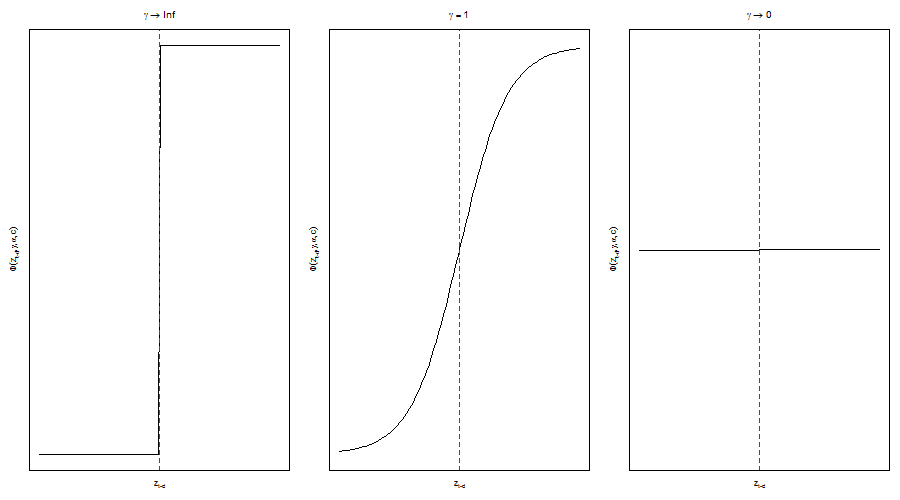
\includegraphics[scale=0.35]{logistic}
\caption{Logistic Transition}
\label{fig:lstar}
\end{figure}
\begin{figure}[ht]
\centering
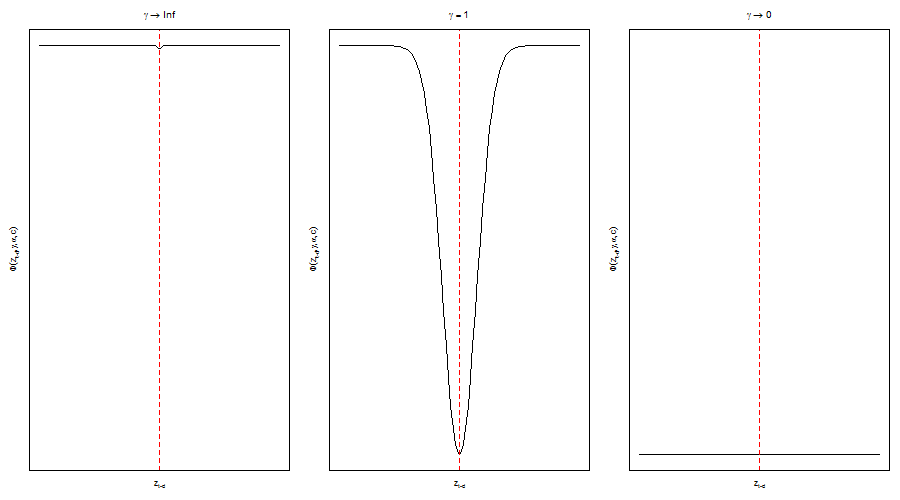
\includegraphics[scale=0.35]{exponential}
\caption{Exponential Transition}
\label{fig:estar}
\end{figure}

By far the most popular test of STAR nonlinearity is described in
\cite{Luukkonen1988} using a Taylor series expansion around equation 
\ref{eq:logistic_cdf}, effectively testing whether $\gamma=0$ (via a auxilliary
regression), which would in turn imply that the $\alpha$ vector is also zero
and hence a rejection of STAR type non-linearity.

An interesting extension considered in this package is the introduction of
autoregressive dynamics in the state equation as follows:
\begin{equation}\label{eq:star_new}
\begin{gathered}
  F\left( {{z_{t - d}};\gamma ,\alpha ,c,\beta } \right) = {\left( {1 + \exp \left\{ { - {\pi _t}} \right\}} \right)^{ - 1}} \hfill \\
  {\pi _t} = \gamma \left( {\alpha '{z_{t - d}} - c} \right) + \beta '\pi _t^{\left( q \right)} \hfill \\
  \pi _t^{\left( q \right)} = {\left( {{\pi _{t - 1}}, \ldots ,{\pi _{t - q}}} \right)^\prime } \hfill \\ 
\end{gathered}
\end{equation}
where the unconstrained state dynamics $\pi_t$ can be initialized by setting
\begin{equation}
\begin{gathered}
  {\pi _0} = \frac{{\gamma \left( {\alpha '{{\bar z}_{t - d}} - c} \right)}}
{{1 - \beta '{\mathbf{1}}}} \hfill \\
  \bar z = {\left( {E\left[ {{z_1}} \right], \ldots ,E\left[ {{z_k}} \right]} \right)^\prime } \hfill \\ 
\end{gathered}
\end{equation}
with a stationarity constraint of $\left| {\sum\limits_{i = 1}^q {{\beta _i}} } \right| < 1$.

This is not just another frivolous extension. Consider that the transition
between states is determined by $z_{t-d}$ which usually arrive as shocks, but
the actual state we are trying to estimate (e.g. recessions) may be more
persistent, in which case the use of AR dynamics may prove usefule. The use of
autoregressive dynamics in the state equation follows related work in the area 
of dynamic binary response models of \cite{Kauppi2008} and \cite{Nyberg2010}.
Generally, estimation becomes quite difficult for more than one autoregressive
parameter in the state dynamics which is why at present only a lag-1
autoregressive state dynamics model is allowed in the package.

The conditional mean dynamics are not limited to AR terms but may include
external regressors (ARX) and moving average (MA) terms in the states giving
rise to a full STARMAX model specification:
\begin{equation}\label{eq:starmax}
\begin{split}
{y_t}& = \left( {{{\phi '}_1}y_t^{\left( p \right)} + {{\xi '}_1}{x_t} +
{{\psi '}_1}e_t^{\left( q \right)}} \right)F\left( {{z_{t - d}};\gamma ,\alpha
,c,\beta } \right)\\
& + \left( {{{\phi '}_2}y_t^{\left( p \right)} + {{\xi '}_2}{x_t} + {{\psi
'}_2}e_t^{\left( q \right)}} \right)\left( {1 - F\left( {{z_{t - d}};\gamma
,\alpha ,c,\beta } \right)} \right) + {\varepsilon _t}\\
\varepsilon _t^{\left( q \right)} &= {\left( {{\varepsilon _{t - 1}}, \ldots
,{\varepsilon _{t - q}}} \right)^\prime },\quad {{\psi '}_i} = {\left(
{{\psi_{i1}},\dots,{\psi _{iq}}} \right)^\prime }\\
{x_t} &= {\left({{x_1},\dots,{x_l}} \right)^\prime },\quad {{\xi'}_1} =
{\left( {{\xi_{i1}},\dots,{\xi _{il}}} \right)^\prime }\\
\end{split}
\end{equation}
Once again, no special notation is used for the lag structure of the $l$
external regressors $x_t$, noting only that these must be passed pre-lagged in the
package's routines. It is also possible that the MA term enters outside of the
states instead of inside giving rise to a STARX with Linear MA terms (STARXLMA):
\begin{equation}
{y_t} = \left( {{{\phi '}_1}y_t^{\left( p \right)} + {{\xi '}_1}{x_t}}
\right)F\left( {{z_{t - d}};\gamma,\alpha,c,\beta } \right) + \left( {{{\phi
'}_2}y_t^{\left( p \right)} + {{\xi '}_2}{x_t}} \right)\left( {1 - F\left(
{{z_{t - d}};\gamma,\alpha,c,\beta } \right)} \right) + \psi 'e_t^{\left( q
\right)} + {\varepsilon _t}
\end{equation}
The STARMAX model therefore encompasses a very wide range of sub-models based on
the type of restrictions placed in the conditional mean and state dynamics, and
choice of switching variables in the latter.\\
A natural question which arises from the representation is whether it is
reasonable to assume that the conditional variance is the same in both states.
Consider the STARMAX 2-state model:
\begin{equation}
\begin{split}
{y_t} &= {\color{red} \left(\phi'_1 y_t^{\left( p \right)} + \xi'_1 x_t +
\psi'_1 e_t^{\left( q \right)} \right)} \left( {\color{blue} F\left( z_{t-d};
\gamma,\alpha , c,\beta \right)}\right) \\
&+ {\color{red} \left( \phi'_2 y_t^{\left( p \right)} + \xi'_2 x_t + \psi'_2
e_t^{\left( q \right)} \right)}\left(1 - {\color{blue} F\left(z_{t-d}; \gamma,
\alpha, c,\beta\right)} \right) + {\varepsilon_t} \\
{\varepsilon_t} &= {y_t} - {\color{red} \left( \mu _{1t} \right)}{\color{blue}
p_t} - {\color{red} \left( \mu _{2t} \right)}\left( 1 -{\color{blue} {p_t}}
\right), d>0\\
\end{split}
\end{equation}
Add and subtract {\color{violet}$y_t p_t $}, and re-arrange:
\begin{equation}\label{eq:starmix}
\begin{gathered}
  {\varepsilon _t} =  {\color{violet}+ {y_t}{p_t}} - {\color{red} \left( \mu _{1t}\right)}{\color{blue} {p_t}} + {y_t} {\color{violet} - {y_t}{p_t}} - {\color{red} \left(\mu _{2t} \right)} \left(1 - {\color{blue}{p_t}} \right)\hfill \\
  {\varepsilon _t} = {\color{violet}+{y_t}{p_t}} - {\color{red}\left( \mu _{1t} \right)}{\color{blue}{p_t}} + {y_t}\left( 1 - {\color{violet}{p_t}} \right) - {\color{red} \left( \mu _{2t} \right)}\left( 1 -{\color{blue} {p_t}} \right) \hfill \\
  {\varepsilon _t} = {\color{red} \left( {y_t} - \mu _{1t} \right)}{\color{blue}{p_t}} + {\color{red}\left( {y_t} - \mu _{2t} \right)}\left(1 - {\color{blue}{p_t}} \right) \hfill \\
  {\varepsilon _t} = {\color{red}\left( \varepsilon _{1,t} \right)}{\color{blue}{p_t}} +{\color{red}\left(\varepsilon _{2,t} \right)}\left(1 - {\color{blue}{p_t}} \right) \hfill \\
 {\color{red} {\varepsilon _{1,t}}} \sim N\left( {0,\sigma _1^2} \right) \hfill {\color{red}{\varepsilon
  _{2,t}}} \sim N\left( {0,\sigma _2^2} \right) \hfill \\
  {\varepsilon _t} \sim N\left( 0,\sigma _1^2{\color{blue}{p_t}} +\sigma _2^2\left(1 - {\color{blue}{p_t}} \right)\right) \hfill \\
\end{gathered}
\end{equation}
Thus, the model can naturally be re-formulated as a mixture of
Normals\footnote{Or any other location-scale invariant distribution} with mixing
probabilities derived from the state dynamics. This provides for a more
parsimonious and clear extension than using GARCH dynamics on the mixed state 
residuals. Alternatively, it can be thought of as the time-invariant version of 
a STARX-STGARCH model with common transition dynamics (and restriction
ARCH=GARCH=0).

\subsection{Multiple States}
\cite{Dijk1999} considered an extension of the 2-state STAR model in equation
\ref{eq:star_original} to a 4-state models as follows:
\begin{equation}\label{eq:mrstar_original}
\begin{split}
{y_t} &= \left[ {{{\phi '}_1}y_t^{\left( p \right)}\left( {1 - F\left( {{z_{t - d}};{\gamma _1},\alpha ,c} \right)} \right) + {{\phi '}_2}y_t^{\left( p \right)}\left( {1 - F\left( {{z_{t - d}};{\gamma _1},\alpha ,c} \right)} \right)} \right]\left( {1 - F\left( {{z_{t - d}};{\gamma _2},b,d} \right)} \right)\\
&+\left[ {{{\phi '}_3}y_t^{\left( p \right)}\left( {1 - F\left( {{z_{t - d}};{\gamma _1},\alpha ,c} \right)} \right) + {{\phi '}_4}y_t^{\left( p \right)}\left( {1 - F\left( {{z_{t - d}};{\gamma _1},\alpha ,c} \right)} \right)} \right]F\left( {{z_{t - d}};{\gamma _2},b,d} \right) + {\varepsilon _t}\\
\end{split}
\end{equation}
This effectively models 2 unique states and one interaction state:
\begin{equation}
\begin{gathered}
  {\mu _1} = {{\phi '}_1}y_t^{\left( p \right)}\left( {1 - F\left( {{z_{t - d}};{\gamma _1},\alpha ,c} \right) - F\left( {{z_{t - d}};{\gamma _2},b,d} \right) + F\left( {{z_{t - d}};{\gamma _1},\alpha ,c} \right)F\left( {{z_{t - d}};{\gamma _2},b,d} \right)} \right) \hfill \\
  {\mu _2} = {{\phi '}_2}y_t^{\left( p \right)}\left( {1 - F\left( {{z_{t - d}};{\gamma _1},\alpha ,c} \right) - F\left( {{z_{t - d}};{\gamma _2},b,d} \right) + F\left( {{z_{t - d}};{\gamma _1},\alpha ,c} \right)F\left( {{z_{t - d}};{\gamma _2},b,d} \right)} \right) \hfill \\
  {\mu _3} = {{\phi '}_3}y_t^{\left( p \right)}\left( {F\left( {{z_{t - d}};{\gamma _2},b,d} \right) - F\left( {{z_{t - d}};{\gamma _1},\alpha ,c} \right)F\left( {{z_{t - d}};{\gamma _2},b,d} \right)} \right) \hfill \\
  {\mu _4} = {{\phi '}_4}y_t^{\left( p \right)}\left( {F\left( {{z_{t - d}};{\gamma _2},b,d} \right) - F\left( {{z_{t - d}};{\gamma _1},\alpha ,c} \right)F\left( {{z_{t - d}};{\gamma _2},b,d} \right)} \right) \hfill \\
\end{gathered}
\end{equation}
Alternatively, the implementation followed in this package takes a page out of
multinomial regression and models multiple states using the softmax function:
\begin{equation}\label{eq:mrstar_new}
{y_t} = \sum\limits_{i = 1}^s {\left[ {\left( {{{\phi '}_i}y_t^{\left( p
\right)} + {{\xi '}_i}{x_t} + {{\psi '}_i}e_t^{\left( q \right)}}
\right){F_i}\left( {{z_{t-d}};{ \gamma_i},{ \alpha _i},{c_i},{\beta_i}}
\right)} \right]}  + {\varepsilon_{i,t}}
\end{equation}
with s-1 distinct states modelled:
\begin{equation}
\begin{gathered}
  {F_i}\left( {{z_{t-d}};{ \gamma_i},{ \alpha _i},{ c_i},{\beta_i}} \right) =
  \frac{{{e^{{\pi _{i,t}}}}}} {{1 + \sum\limits_{i = 1}^{s - 1} {{e^{{\pi _{i,t}}}}} }} \hfill \\
  {F_s}\left( {{z_{t-d}};{ \gamma_i},{ \alpha _i},{ c_i},{\beta_i}} \right) =
  \frac{1} {{1 + \sum\limits_{i = 1}^{s - 1} {{e^{{\pi _{i,t}}}}} }} \hfill \\
\end{gathered}
\end{equation}
where the $s$ states are weighted to sum to unity. This appears, at least to
this author, to be a more natural representation for a multi-state setup. In the
\textbf{twinkle} package, upto 4 states may be modelled\footnote{For the case of
only a single state, it is also possible to pass a set of 'time' weights.}

\subsection{Estimation}
Estimation of the STARMAX models is done by maximizing the likelihood without
imposing any particular inequality restrictions on the state dynamic intercepts
or any parameter bound restrictions (except for positivity bounds on the
variance and $\gamma$ state scaling parameter).\footnote{Constraints on the
autoregressive and moving average parameters may also be placed to impose some
type of stationarity constraint per state.} Since unconstrained optimizers
appear to do quite well for hard nonlinear/non-smooth problems, the main solver
in the twinkle package is the BFGS solver from the optim function. It is
possible to include parameter bounds in which case a logistic transformation is
used with the unconstrained solvers.
Additional solvers included are 'nlminb' (bound constrained), 'solnp'
(nonlinear SQP solver with nonlinear constraints), 'cmaes' (bound constrained
global solver) and 'deoptim' (bound constrained global solver).
However, it is suggested that either a multi-start strategy is followed
(by choosing 'msoptim') or an iterative search strategy ('strategy') which
cycles between fixing the state parameters to estimate the conditional mean 
parameters (linear), fixing the conditional mean parameters to estimate the
state parameters (nonlinear) and a random start estimation. As with general
nonlinear optimization problems, scaling of the data prior to estimation
may help, an ica or pca transformation if they are highly correlated, or hinge
basis transformation of the dataset via the earth package is another interesting
option in the case of relevant feature extraction.
\section{Forecasting}\label{sec:2}
Consider a general nonlinear first order autoregressive model:
\begin{equation}\label{eq:nonlinar1}
{y_t} = F\left( {{y_{t - 1}};\theta } \right) + {\varepsilon _t}
\end{equation}
where $ F\left( {{y_{t - 1}};\theta } \right)$ is some nonlinear function 
mapping $y_{t-1}$ to $y_t$ given the parameter set $\theta$. The optimal h-step
ahead  point forecast, using a least squares criterion, of $y_{t+h}$ at time $t$
is given by:
\begin{equation}
{{\hat y}_{t + h\left| t \right.}} = E\left[ {{y_{t + h}}\left| {{\Im _t}} \right.} \right]
\end{equation}
where $\Im_t$ is the information set upto time $t$. Given  that $E\left[
{{\varepsilon_{t + 1}}\left| {{\Im _t}} \right.} \right] = 0$, then the
1-step-ahead optimal forecast is:
\begin{equation}
{{\hat y}_{t + 1\left| t \right.}} = E\left[ {{y_{t + 1}}\left| {{\Im _t}} \right.} \right] = F\left( {{y_t};\theta } \right)
\end{equation}
which is the same as when $F(.)$ is linear. However, for horizons greater than
1, this is not the case since $E\left[ {F\left( . \right)} \right] \ne F\left(
{E\left[ . \right]} \right)$,  which means that simple recursive relationship 
found in the linear case do not exist in the nonlinear case. Instead, consider
the  h-step-ahead point forecast using the following closed form 
representation:\footnote{This is based on the Chapman-Kolmogorov relation:
\begin{equation}
g\left( {{y_{t + h}}\left| {{\Im _t}} \right.} \right) = \int_{ - \infty }^\infty  {g\left( {{y_{t + h}}\left| {{y_{t + h - 1}}} \right.} \right)g\left( {{y_{t + h - 1}}\left| {{\Im _t}} \right.} \right)d{y_{t + h - 1}}}
\end{equation}
which leads to Equation \ref{eq:hstepforecast} after taking conditional expectations from both sides.
}
\begin{equation}\label{eq:hstepforecast}
E\left[ {{y_{t + h}}\left| {{\Im _t}} \right.} \right] = \int_{ - \infty }^\infty  {E\left[ {{y_{t + h}}\left| {{y_{t + h - 1}}} \right.} \right]g\left( {{y_{t + h - 1}}\left| {{\Im _t}} \right.} \right)d{y_{t + h - 1}}}
\end{equation}
where $g\left( {{y_{t + h}}\left| {{\Im _t}} \right.} \right) = f\left( {{y_{t + h}} - F\left( {{y_{t + h - 1}};\theta } \right)} \right)$, is the distribution of the shock $\varepsilon_{t+h}$ with mean $F\left( {y_{t + h - 1}}\right)$, though the distribution $\varepsilon_t$ is never known with certainty.
A number of approaches have been used in the literature to estimate this
integral. It is simple to see that the conditional distribution of ${g\left(
{{y_{t + h - 1}}\left| {{\Im _t}} \right.} \right)}$ can be obtained recursively
starting at h=2 and noting that $g\left( {{y_{t + 1}}\left| {{\Im _t}} \right.}
\right) = f\left( {{y_{t + 1}} - F\left( {{y_t};\theta } \right)} \right)$. To
obtain the forecasts, numerical integration can be used (applied recursively) or
monte carlo methods. In the former case, the form of the conditional
distribution $f\left( {.\left| {{\Im _t}} \right.} \right)$ can be replaced by a
kernel estimator, whereas in the latter case one has an option of using an
empirical bootstrap, simulating from the conditional distribution $f\left(
{.\left| {{\Im _t}} \right.} \right)$ or a kernel estimator. For instance,  
the 2-step ahead monte carlo forecast is given by:
\begin{equation}
{{\hat y}_{t + 2\left| t \right.}} = \frac{1}{T}\sum\limits_{i = 1}^T {F\left( {{{\hat y}_{t + 1\left| t \right.}} + {\varepsilon _i};\theta } \right)}
\end{equation}
However, in the case when a GARCH model is used for the modelling of the
conditional variance, then the monte carlo forecast needs to be adjusted as follows:
\begin{equation}
{{\hat y}_{t + 2\left| t \right.}} = \frac{1}{T}\sum\limits_{i = 1}^T {F\left( {{{\hat y}_{t + 1\left| t \right.}} + {z_i}{{\hat \sigma }_{t + 2\left| t \right.}};\theta } \right)}
\end{equation}
where $z_i$ represent draws from either the parametric standardized distribution
of the model  or the standardized in-sample innovations (or draws from a kernel
estimated density of the standardized in-sample innovations), which are then
multiplied  by the forecast GARCH volatility ${{{\hat \sigma }_{t + 2\left| t
\right.}}}$ to obtain the forecast residuals $\varepsilon_i$.
One benefit of using a monte-carlo or bootstrap approach is that they
immediately give rise to the density of each point forecast thus allowing for
the creation of interval forecasts.

%\section{Simulation}\label{sec:3}
%The key issue considered in the implementation of a simula

%\section{Generalized Impulse Response}\label{sec:4}

\pagebreak
\section{Software Implementation}\label{sec:5}
\subsection{Specification}
The entry point to defining and estimating a STARMAX model in the twinkle
package is the starspec function:
\begin{Schunk}
\begin{Sinput}
>starspec
\end{Sinput}
\begin{Soutput}
function(
mean.model = list(states=2, include.intercept=c(1,1), arOrder=c(1,1), 
	maOrder=c(0, 0), matype="linear", statevar=c("y","s"), s=NULL, 
	statear=FALSE, ylags=1, xreg=NULL, yfun=NULL, transform="log"), 
variance.model=list(dynamic=FALSE, model="sGARCH", garchOrder=c(1,1), 
	submodel=NULL, vreg=NULL, variance.targeting=FALSE), 
distribution.model="norm", start.pars=list(), fixed.pars=list(), 
fixed.prob=NULL, ...)
\end{Soutput}
\end{Schunk}
The \textbf{mean.model} defines the equation for the conditional mean dynamics
including the state dynamics. Upto 4 \textbf{states} are allowed, with the
1-state option having a special implementation in that the \textbf{fixed.probs}
list is an xts matrix (alined to the dataset which will be passed to the
estimation routine) of weights. By default this is set to a vector of ones in
this case but may be any other 'time-weighting' scheme the user wishes. The
options for \textbf{intercept}, \textbf{arOrder} and \textbf{maOrder} should be
integer vectors of length equal to the number of \textbf{states}. 

The \textbf{matype} denotes whether the moving average terms enter inside the
states ('states') or outside ('linear'). 

The \textbf{statevar} indicates whether the model will switch based on its own
value ('y') or an exogenouse set of regressors ('s'), in which case an xts 
matrix (aligned to the index of the dataset and appropriately lagged) is passed 
to \textbf{s}. In the case that \textbf{statevar} is 'y', then \textbf{ylags} 
is an integer vector of the unique lags to use as a linear combination. 

The \textbf{yfun}  option allows the user to pass a function to transform the 
value of y\footnote{The function must return the same length as the value  it
receives without any NAs or NaNs.} prior to being used in the state dynamics 
equation. While it may appear at first that the same can be achieved by passing 
a pre-transformed value and using 's' as the \textbf{statevar}, consider that
simulation and n-ahead forecasts (which depend on simulation methods) on 
transformed values of 'y' can then be used directly, where it would have been
impossible to do so otherwise (because of the path dependency). 

The \textbf{xreg} is an optional xts matrix of external regressors which needs
to be aligned to the index of the dataset (and appropriately lagged). The
\textbf{statear} indicates whether to include lag-1 autoregression in the state
dynamics as discussed previously in equation \ref{eq:star_new}.

Tthe \textbf{transform} is currently fixed to use only the logistic
transformation, and there are no plans to extend to the exponential at present.

The variance model can be \textbf{dynamic}, in which case a choice of
'mixture','sGARCH','gjrGARCH' and 'eGARCH' are implemented, else by default a
static variance model is used. For the GARCH flavors, the rest of the options
follow from the rugarch package, whilst the 'mixture' model is based on 
equation \ref{eq:starmix}. 

All distributions implemented in rugarch are included as options in
\textbf{distribution.model}, while fixed and starting parameters can be passed
directly via \textbf{fixed.pars} and \textbf{start.pars} respectively, else
later on via the \textbf{setfixed<-} and \textbf{setpars<-} methods on the star
specification (note that there is also a \textbf{setbounds<-}  methods for
setting and enforcing parameter bounds).

Finally, the \textbf{fixed.probs} list allows the user to pass an xts matrix of 
fixed probabilities for each state (aligned to the index of the dataset and with
columns equal to \textbf{states}). This could for instance be the forecast
probabilities from another model (e.g. logistic regression) representing market
up and down periods, recessions etc. In this case the state equation is not used
and the model is effectively linear and extremely fast to estimate for
the conditional mean dynamics.

The returned specification object is of class \textbf{STARspec} which may be
passed to the estimation routine \textbf{starfit}. If the object has been
assigned fixed parameters for the complete parameter set, then it may instead be
passed to the \textbf{starfilter}, \code{starforecast} or the \textbf{starpath}
routines.

\subsection{Estimation}
Once the model has been specified, it may be estimated by maximum likelihood
using the \code{starfit} routine:
\begin{Schunk}
\begin{Sinput}
>starfit
\end{Sinput}
\begin{Soutput}
(spec, data, out.sample=0, solver="optim", solver.control=list(), 
fit.control=list(stationarity=0, fixed.se=0, rec.init="all"), 
cluster=NULL, n=25, ...)
\end{Soutput}
\end{Schunk}
The \textbf{data} must be an xts object with the same time indices as any data
already passed to the \code{STARspec} object and contain only numeric data
without any missing values. The \textbf{out.sample} is used to indicate how many
data points to optionally leave out in the estimation (from the end of the
dataset) for use in out-of-sample forecasting later on when the estimated object
is passed to the \code{starfilter} routine. Perhaps the most important choice
to be made is the type of \textbf{solver} to use and it's control parameters
(\textbf{solver.control}). The following solvers and 'strategies' are included:
\begin{itemize}
  \item optim. The preferred choice is the BFGS solver. The choice of solver is
  controlled by the \emph{method} option in the \textbf{solver.control} list.
  \item nlminb. Have had little luck getting the same performance as the BFGS
  solver.
  \item solnp. Will most likely find a local solution.
  \item cmaes. Even though it is a global solver, it requires careful tweaking
  of the control parameters (and there are many). This is the parma package
  version of the solver.
  \item deoptim. Another global solver. May be slow and require tweaking of the
  control parameters.
  \item msoptim. A multistart version of optim with option for using the
  \textbf{cluster} option for parallel evaluation. The number of
  multi-starts is controlled by the \emph{n.restarts} option in the
  \textbf{solver.control} list.
  \item strategy. A special purpose optimization strategy for STAR problems
  using the BFGS solver. It cycles between keeping the state variables fixed and
  estimating the linear variables (conditional mean, variance and any
  distribution parameters), keeping the linear variables fixed and estimating
  the state variables, and a random re-start optimization to control for
  possibly local solutions. The argument \textbf{n} in the routine controls the
  number of times to cycle through this strategy. The \textbf{solver.control}
  list should pass control arguments for the BFGS solver. This is somewhat
  related to concentrating the sum of squares methodology in terms of the
  estimation strategy, but does not minimize the sum of squares.
\end{itemize}
The \emph{strategy} and \emph{msoptim} solver strategies should be the preferred
options when estimating STARMA models.

The resulting object of class \code{STARfit} has a number of methods including
an S4 summary (\emph{show}) and a number of S4 extractor methods such as
\code{coef}, \code{likelihood}, \code{vcov}, \code{infocriteria},
\code{modelmatrix}, \code{quantile}, \code{pit}, \code{fitted}, \code{residuals}
and \code{sigma}.
A new method \code{states} can be used for extracting the conditional state
probabilities, with an extra argument \textbf{type} with options for 'prob' 
(probabilties), 'condm' (conditional mean dynamics per state) and anything else 
will return the untransformed (raw) state dynamics. The methods are documented
in the help page of \code{STARfit-class}. A default \code{plot} method is also
available which plots the states and fitted values of the model.
Finally, note that unlike other implementations which start the iteration (and
summation of the likelihood) of the model at the maximum of the AR or MA lags,
the \textbf{twinkle} package starts at T=1 and builds up the likelihood by
using all information available at that point (e.g. for T=1, if an intercept is
included then that is used to obtain the residuals, then at T=2, the AR1
parameter is used and so on). For the \textbf{nonlinearTest} in section
\ref{sec:6} the lags are first substracted before carrying out the test in 
order to be consistent with published results.

\subsection{Filtering}
An object of class \code{STARspec} with pre-assigned fixed parameter values
(for the complete model parameter set) may be passed to the \code{starfilter}
routine with a new or augmented dataset (to that which was used to estimate the
original parameters). In this way, new data can be filtered using existing
parameters which is equivalent to performing rolling 1-step ahead forecasts
(without re-estimation).
\begin{Schunk}
\begin{Sinput}
>starfilter
\end{Sinput}
\begin{Soutput}
(spec, data, out.sample=0, n.old=NULL, rec.init="all", ...) 
\end{Soutput}
\end{Schunk}
It is probably best to provide an augmented dataset for filtering since the
model may depend on the complete history (particularly as regards use of the
autoregressive parameter in the state dynamics), in which case the
\textbf{n.old} option should also be used to denote the size of the original
dataset.

\subsection{Forecasting}
Forecasting can be carried out either from an estimated object of class
\code{STARfit} or a specification with fixed parameters of class
\code{STARspec} (in which case the \textbf{data} argument must also be
used\footnote{Effectively, the data is filtered with the fixed parameter
specification prior to the forecast being carried out}).
\begin{Schunk}
\begin{Sinput}
>starforecast
\end{Sinput}
\begin{Soutput}
function(fitORspec, data=NULL, n.ahead=1, n.roll=0, out.sample=0, 
external.forecasts=list(xregfor=NULL, vregfor=NULL, sfor=NULL, 
probfor=NULL), method=c("an.parametric", "an.kernel", "mc.empirical", 
"mc.parametric", "mc.kernel"), mc.sims=NULL, ...) 
\end{Soutput}
\end{Schunk}
As discussed in Section \ref{sec:2}, for n-step (n>1) ahead forecasts,
there are a number of options available based on recursive quadrature
integration ('an') of the integral in Equation \ref{eq:hstepforecast} 
else monte carlo ('mc') integration. The \emph{parametric} method uses
the density from the estimated object while the \emph{kernel} method fits
a kernel density to the residuals. Finally, and only available for the monte
carlo method, the \emph{empirical} option samples from the empirical
distribution of the residuals. Clearly with a limited history it may be optimal
to use either the \emph{parametric} or \emph{kernel} methods. For the monte
carlo integration, the \textbf{mc.sims} argument denotes the number of samples
to use per period.

Some care should be taken when passing \textbf{external.forecasts} for the
conditional mean regressors (xregfor), the conditional variance regressors
(vregfor), the conditional state dynamics regressors (sfor) and the conditional
probability (probfor) in the case that the state probabilities where passed as
fixed in the specification. These xts matrices should be pre-lagged in the same
way as the input matrices where in the specification.

The resulting object is of class \code{STARforecast} with a number of extractor
functions documented in the help page of the class and similar to those
available for the \code{STARfit} class. Of particular interest in the case of
monte carlo integration is the estimated density of each point forecast which
may be extracted from the object.

\subsection{Simulation}
Simulation can be carried out either directly on a \code{STARfit} object using
the \code{starsim} routine, else on a \code{STARspec} object with fixed
parameters using the \code{starpath} method.

\begin{Schunk}
\begin{Sinput}
>starsim
\end{Sinput}
\begin{Soutput}
function(fit, n.sim=1000, n.start=0, m.sim=1, presigma=NA, prereturns=NA, 
preresiduals=NA, rseed=NA, custom.dist=list(name=NA, distfit=NA), 
xregsim=NULL, vregsim=NULL, ssim=NULL, probsim=NULL, ...)
\end{Soutput}
\end{Schunk}
The arguments follow similar convention as in related packages. In particular,
the \textbf{ssim} argument should be a list of matrices for the
simulated values of the external regressors (\textbf{s}) in the state dynamics,
while \textbf{probsim} should be a list of matrices of the simulated state
probabilities in the case that fixed probabilties were used in the original
specification.
\\
Similarly, the \code{starpath} routine has the following arguments:
\begin{Schunk}
\begin{Sinput}
>starpath
\end{Sinput}
\begin{Soutput}
function(spec, n.sim=1000, n.start=0, m.sim=1, presigma=NA, prereturns=NA, 
preresiduals=NA, rseed=NA, custom.dist=list(name=NA, distfit=NA), 
xregsim=NULL, vregsim=NULL, ssim=NULL, probsim=NULL, ...)
\end{Soutput}
\end{Schunk}
Where the \textbf{prereturns} are now required as depending on the model, so is
\textbf{presigma} and \textbf{preresiduals}. The length of these initialization
matrices is determined by the maximum of the conditional state, mean and
variance dynamic lags.

\section{Mispecification Test}\label{sec:6}
\subsection{STAR type nonlinearity}
The key test of STAR type nonlinearity is that of \cite{Luukkonen1988} which
is implemented in the \code{nonlinearTest} method. This effectively tests the
null hypothesis that the model is linear against STAR type nonlinearity. 
Because of the presence of unidentified\footnote{Under the null, $\gamma$ is 
zero and hence the transition probabilities collapse to 0.5, in which case $c$
and $alpha$ (and $beta$ if that is used) are not identified.} STAR model 
parameters under the null, the test replaces the logistic transition function 
with a third order Taylor series approximation around $\gamma=0$ leading to the
following equation:
\begin{equation}
{y_t} = \text{const}+{{\mathbf{X}}_t}{\beta _0} + {{\mathbf{X}}_t}{z_t}{\beta
_1} + {{\mathbf{X}}_t}z_t^2{\beta _1} + {{\mathbf{X}}_t}z_t^3{\beta _1} + {\varepsilon _t}
\end{equation}
where ${{\mathbf{X}}_t} = {\left( {\tilde y_t^{\left( p \right)},{{\tilde
x}_t}} \right)^\prime }$ is the vector of lagged series and external variables
as in equation \ref{eq:starmax}, and $z_t$ is the state transition variable. In
the case that this is a vector then it is not clear what one should do since
only under a single variable does the identification restriction allow the test
to be carried out without the model having to be estimated. In the package this
case is dealt with by multiplying the $z_t$ vector of $k$ transition variables
by the estimated coefficient vector $\alpha=(1,\alpha_2,\ldots,\alpha_k)$, which
means that the model needs to be estimated first. Additionally, in the case that
this vector is made up of external variables rather than a lagged vector of the
series ($y_t$), then a constant is added to the $\mathbf{X}$ vector in the cases
that it is multiplied by $z_t$ so that ${{\mathbf{X}}_t} = {\left(1, {\tilde
y_t^{\left( p \right)},{{\tilde x}_t}} \right)^\prime }$. This is not possible
in the case of $z_t$ being the lagged series of $y_t$ since a constant would
induce almost perfect multicollinearity.
The test can be run on either an estimated object of class \textbf{STARfit} or a
specification object of class \textbf{STARspec} in which case a data object of
class \textbf{xts} is also required. The test returns both the $\chi^2$ and $F$
distribution statistics and p-values, and there is also an option for computing
\emph{robust} (to heteroskedasticity) statistics based on the procedure
described in \cite{Granger1993}.

\section{Examples}\label{sec:7}
In this section, a small number of examples are considered in order to
illustrate the working of the package. A detailed testing suite is available in
the src distribution under the \textbf{inst} folder.

\subsection{The Dutch Gilder Benchmark (\cite{Franses2000})}
The package contains the \code{forex} dataset which is an xts matrix
consisting of the daily value of 8 currency pairs spanning the period
31-12-1979 to 31-12-1998 from the book of \cite{Franses2000}, and originally
sourced from the Federal Reserve Bank of New York. In Chapter 3 of their book,
they provide a model for the Dutch Gilder weekly (Wednesday) series using a
STAR model with switching based on the 4-week moving average of the lagged
absolute value of this return series. In this example we replicate their
results, making use of the custom transformation function \emph{yfun}.
\begin{Schunk}
\begin{Sinput}
require(quantmod)
data(forex)
# to replicate the results of van Dijk and Franses use:
# next observation carried backward (i.e. fromLast=TRUE)
# for missing values
fx = na.locf(forex, fromLast = TRUE)
fxw = fx[which(weekdays(index(forex))=="Wednesday"),4]
dx = ROC(fxw, na.pad=FALSE)*100
# threshold variable a running mean of the absolute returns
# period considered
idx = 1:521
fun = function(x){
x = as.numeric(x)
y = runMean(abs(x), n=4)
y[1:3] = c(abs(x[1]), mean(abs(x[1:2])), mean(abs(x[1:3])))
return(y)
}
spec = starspec(mean.model = list(states=2, include.intercept=c(1,1), 
arOrder=c(0,2), statevar="y",ylags=1,yfun=fun))
control=list(alpha=1, beta=0.4, gamma=1.2, reltol=1e-12, trace=1,
method="BFGS",n.restarts=3)
fit = starfit(spec, data=dx[idx], solver="msoptim", solver.control=control)
twinklepars = coef(fit)
vdfpars = c(-0.18019807, 0.05980984, 0.28705073, 0.21335697, 4.3161180, 1.3554227)
vdfse   = c( 0.13140430, 0.10138187, 0.10719107, 0.10026741, 1.0771948, 0.1521352)
names(vdfpars) = names(vdfse) = c("s1.phi0", "s2.phi0", "s2.phi1","s2.phi2",
"s1.gamma", "s1.c") twinklepars = coef(fit1)
twinklese = sqrt(diag(vcov(fit, robust=FALSE)))
twinkleSSE = sum(residuals(fit)^2)
vdfSSE = 1233.321352
\end{Sinput}
\begin{Soutput}
>print(data.frame(vdfpars = vdfpars, twinklepars = twinklepars[1:6]))
             vdfpars twinklepars
s1.phi0  -0.18019807 -0.17894764
s2.phi0   0.05980984  0.07028044
s2.phi1   0.28705073  0.29665768
s2.phi2   0.21335697  0.21808028
s1.gamma  4.31611800  7.96823137
s1.c      1.35542270  1.34296993

>print(data.frame(vdfse = vdfse, twinklese = twinklese[1:6]))
             vdfse  twinklese
s1.phi0  0.1314043 0.14132956
s2.phi0  0.1013819 0.09597175
s2.phi1  0.1071911 0.11585311
s2.phi2  0.1002674 0.10842124
s1.gamma 1.0771948 5.54362697
s1.c     0.1521352 0.19176212

>show(fit)
*---------------------------------*
*          STAR Model Fit         *
*---------------------------------*
states       : 2
statevar     : y
statear      : FALSE
variance     : static
distribution : norm


Optimal Parameters (Robust Standard Errors)
------------------------------------
           Estimate  Std. Error  t value Pr(>|t|)
s1.phi0    -0.17895    0.192527 -0.92947 0.352647
s2.phi0     0.07028    0.082826  0.84854 0.396140
s2.phi1     0.29666    0.119232  2.48806 0.012844
s2.phi2     0.21808    0.119800  1.82037 0.068703
s1.gamma    7.96823    3.967261  2.00850 0.044590
s1.c        1.34297    0.260680  5.15180 0.000000
s1.alpha1   1.00000          NA       NA       NA
sigma       1.54011    0.057506 26.78179 0.000000

LogLikelihood : -964.2643 
                   
Akaike       3.7285
Bayes        3.7856
Shibata      3.7281
Hannan-Quinn 3.7509

r.squared         :  0.0418
r.squared (adj)   :  0.0287
RSS               :  1235.787
skewness (res)    :  -0.47002
ex.kurtosis (res) :  0.88495

AR roots
         Moduli1 Moduli2
state_1       NA      NA
state_2 1.566636 2.92695
\end{Soutput}
\end{Schunk}
\begin{figure}
\centering
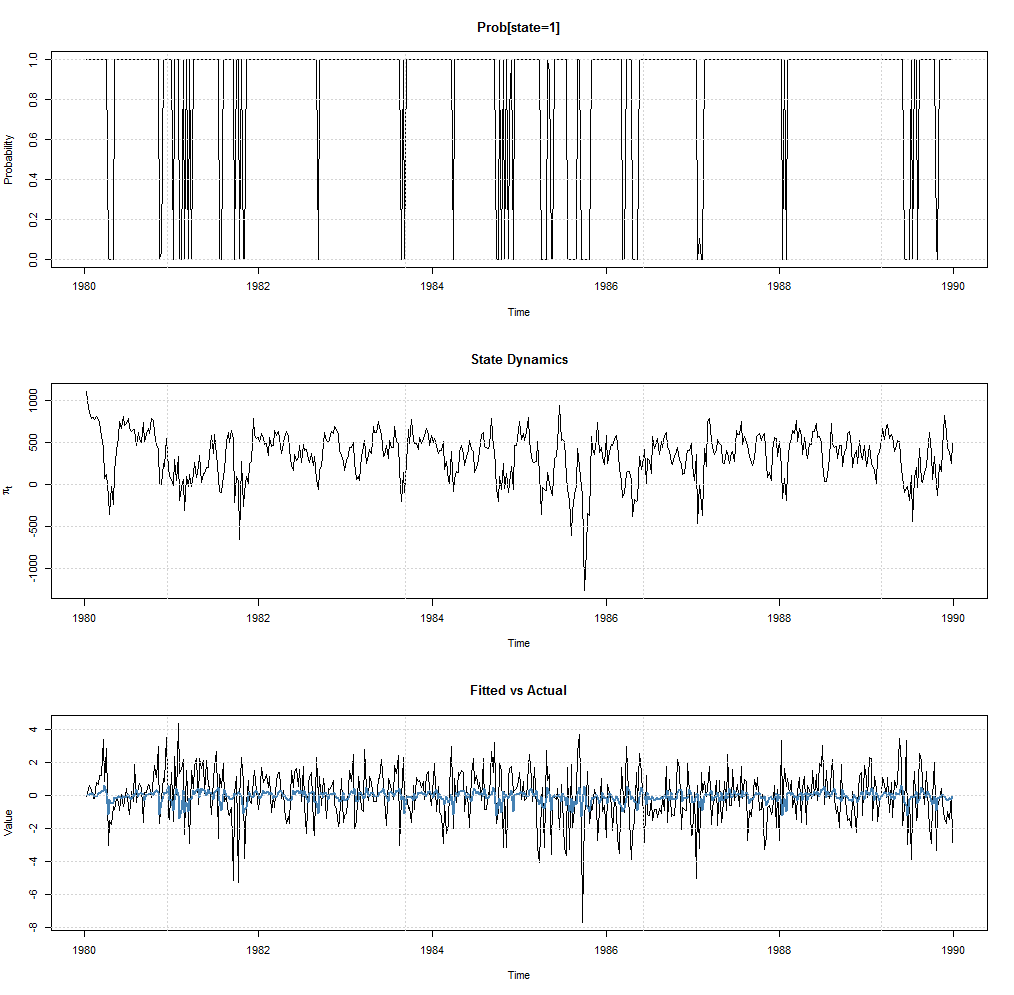
\includegraphics[scale=0.2]{fx_plot}
\caption{Dutch Gilder STAR Model}
\label{fig:guilder}
\end{figure}
There is also a default plot method which creates 3 panels to show the estimated
state probabilities, raw state dynamics and fitted versus actual as shown in
figure \ref{fig:guilder}. There is also a transition probability plot
\emph{trans2fun2d} as shown in figure \ref{fig:transition}. The threshold value
at which state switching occurs is about 1.8. Given the scaling of the original 
input data, and the coefficient summary, this means that when average 4 week 
absolute returns are above 1.8\% the states switch from a high (positive) to a
low (negative) state.

\begin{figure}
\centering
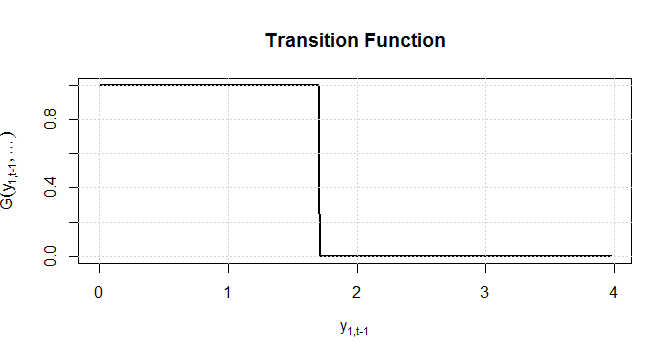
\includegraphics[scale=0.2]{fx_trans}
\caption{Dutch Gilder Transition}
\label{fig:transition}
\end{figure}

\subsection{Nasdaq 100 Index Benchmark}
The package has a second dataset of the OHLCV of the Nasdaq 100 index spanning
the period \emph{02-01-1996} to \emph{12-10-2001} from Yahoo finance. This
is the same dataset used in a number of examples in the excellent book of
\cite{Zivot2007}. The example here is taken from chapter 18 of that book based
on a 'realized' weekly variance measure.
\begin{figure}[ht]
\centering
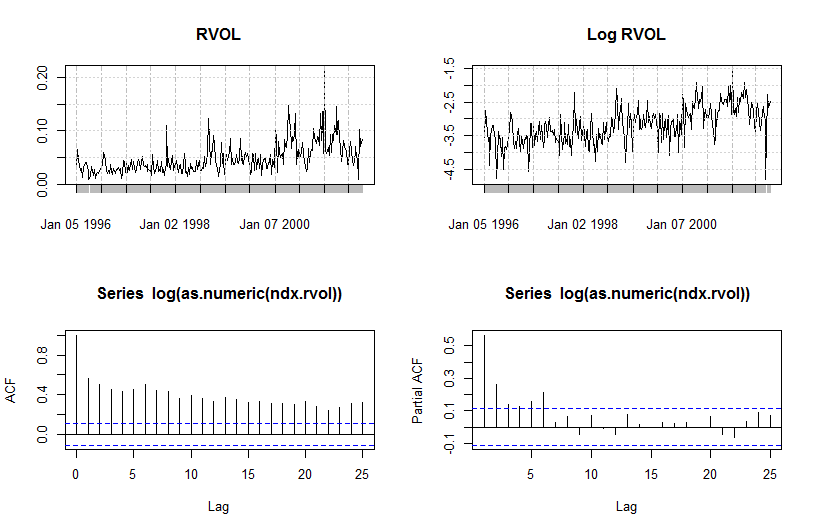
\includegraphics[scale=0.35]{ndxplot}
\caption{Nasdaq 100 Realized Volatility}
\label{fig:ndx}
\end{figure}
\begin{Schunk}
\begin{Sinput}
load(ndx)
require(quantmod)
ndx.ret2 = ROC(Cl(ndx), na.pad=FALSE)^2
ndx.rvol = sqrt(apply.weekly(ndx.ret2, FUN=sum))
colnames(ndx.rvol) = "RVOL"
par(mfrow=c(2,2))
plot(ndx.rvol, main="RVOL")
plot(log(ndx.rvol), main="Log RVOL")
ndx.acf = acf(log(as.numeric(ndx.rvol)), 25)
ndx.pacf = pacf(log(as.numeric(ndx.rvol)), 25)
spec = starspec(mean.model=list(states=2,arOrder=c(2,2),
statevar="y",ylags=1))
nt1 = nonlinearTest(spec, data=log(ndx.rvol))
nt2 = nonlinearTest(spec, data=log(ndx.rvol), robust=TRUE)
testmat = matrix(NA, ncol=4, nrow=2)
colnames(testmat) =c("F-stat","p-value","Chisq-stat","pvalue")
rownames(testmat) =c("standard","robust")
testmat[1,]=c(nt1$F.statistic,nt1$F.pvalue,nt1$chisq.statistic,nt1$chisq.pvalue)
testmat[2,]=c(nt2$F.statistic,nt2$F.pvalue,nt2$chisq.statistic,nt2$chisq.pvalue)
print(testmat)
\end{Sinput}
\begin{Soutput}


           F-stat     p-value Chisq-stat      pvalue
standard 3.708895 0.001436576   21.31186 0.001612269
robust   2.569438 0.019308720   15.09379 0.019539641
\end{Soutput}
\end{Schunk}
This is the same results as given on P.670 and 680 of the \cite{Zivot2007} book.
Finally, estimate the model:
\begin{Schunk}
\begin{Sinput}
ctrl=list(maxit=15000,alpha=1,beta=0.4,gamma=1.2,reltol=1e-12,method="BFGS")
mod = starfit(spec, data = log(ndx.rvol),
solver="strategy",solver.control=ctrl, n=8)
show(mod)
plot(mod)
\end{Sinput}
\begin{Soutput}
*---------------------------------*
*          STAR Model Fit         *
*---------------------------------*
states       : 2
statevar     : y
statear      : FALSE
variance     : static
distribution : norm

Optimal Parameters (Robust Standard Errors)
------------------------------------
           Estimate  Std. Error   t value Pr(>|t|)
s1.phi0    -3.55151    0.052459 -67.70121 0.000000
s1.phi1    -0.86597    0.296898  -2.91672 0.003537
s1.phi2     0.19690    0.138362   1.42305 0.154721
s2.phi0    -3.71423    2.412406  -1.53964 0.123648
s2.phi1    -0.21872    0.572678  -0.38193 0.702512
s2.phi2     0.21283    0.062668   3.39616 0.000683
s1.gamma    2.74428    1.449708   1.89298 0.058360
s1.c       -2.65726    0.208624 -12.73707 0.000000
s1.alpha1   1.00000          NA        NA       NA
sigma       0.40946    0.021635  18.92585 0.000000

LogLikelihood : -158.8607 
                   
Akaike       1.1117
Bayes        1.2222
Shibata      1.1100
Hannan-Quinn 1.1559

r.squared         :  0.4114
r.squared (adj)   :  0.3932
RSS               :  50.63322
skewness (res)    :  -0.36457
ex.kurtosis (res) :  1.33252

AR roots
          Moduli1  Moduli2
state_1 0.9497038 5.347780
state_2 2.7415442 1.713851
\end{Soutput}
\end{Schunk}
\begin{figure}[ht]
\centering
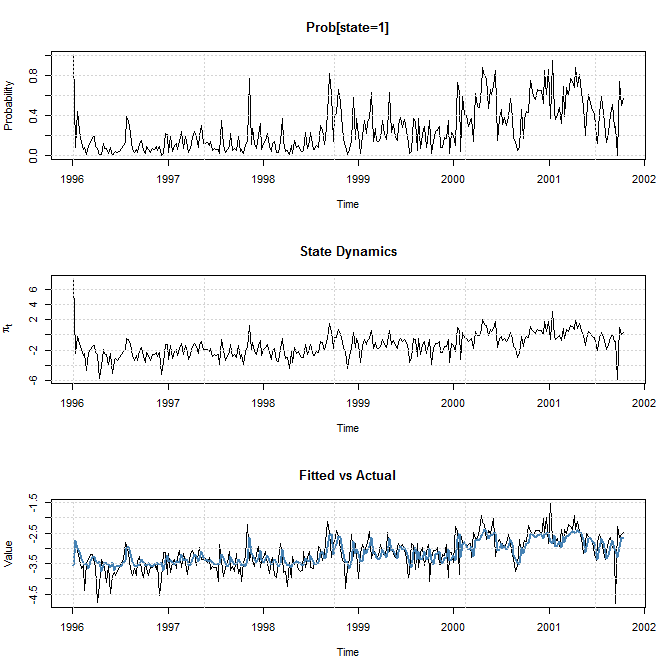
\includegraphics[scale=0.35]{ndxfit}
\caption{Nasdaq 100 Estimated 2-state STAR model}
\label{fig:ndxfit}
\end{figure}